\documentclass[xcolor=dvipsnames]{beamer}
\usepackage{ods}
%\usepackage{ods-figs}
\usepackage[cm]{sfmath}
\usepackage[utf8]{inputenc}
\usepackage{array}
%\usepackage{enumitem}
%\usepackage{enumitem}
%\setitemize{itemsep=1.5ex}
%\setlength{\leftmargini}{0pt}
\usepackage{array}

\newcommand{\caressed}{$\kappa$aressed}
\newcommand{\caresses}{$\kappa$aresses}
\newcommand{\R}{\mathbb{R}}
\newcommand{\dual}[1]{#1^\star}
\newcommand{\Fary}{F\'ary}
\newcommand{\N}{\mathbb{N}}

\DeclareMathOperator{\tw}{tw}
\DeclareMathOperator{\td}{td}
\DeclareMathOperator{\stw}{stw}

\title[$\ell$-vertex ranking]{Asymptotically Optimal Vertex Ranking \newline of Planar Graphs (and Beyond)}
\author[Bose, Dujmović, Javarsineh, M]{Jit Bose \and Vida Dujmović \and Mehrnoosh Javarsineh \and Pat Morin}
\titlegraphic{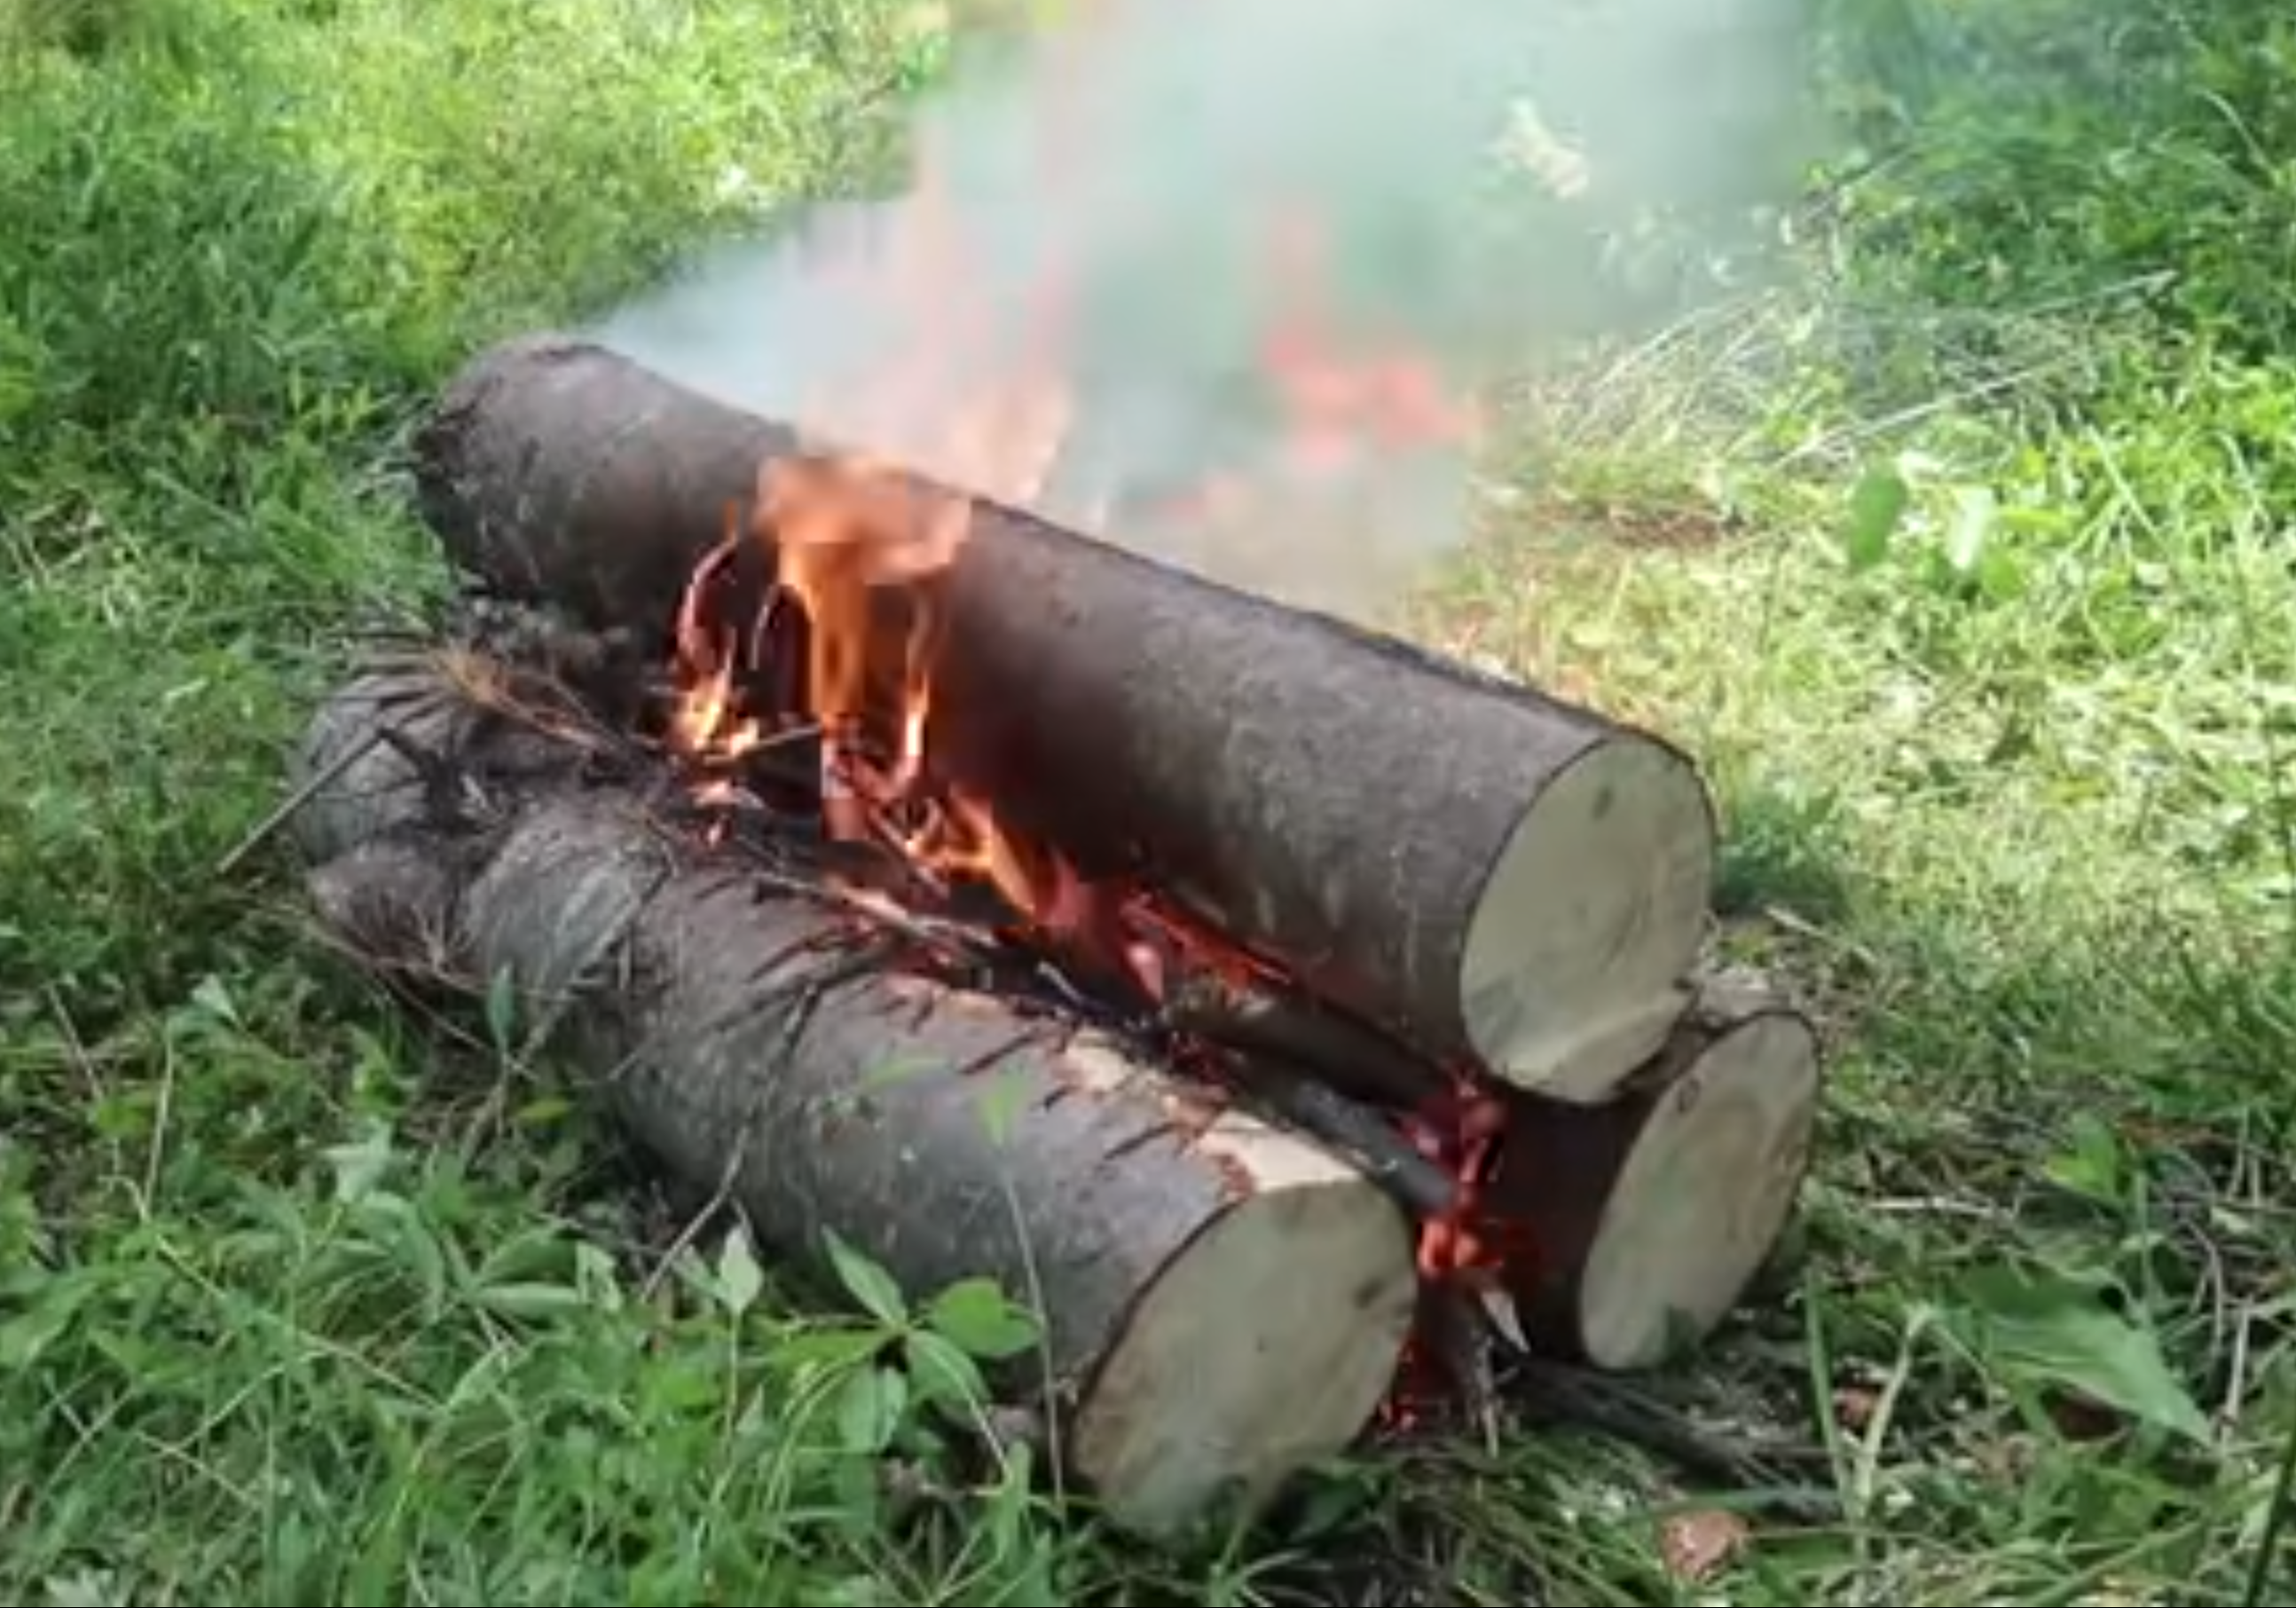
\includegraphics[height=.25\textheight]{images/three-logs.png}}

% 
\includegraphics[height=1em]{by}}

\begin{document}

\begin{frame}
  \titlepage
\end{frame}

% \begin{frame}
%     \frametitle{Outline}
%
%     \tableofcontents
% \end{frame}


\section{Vertex ranking, centered colouring and treedepth}

\begin{frame}
  \frametitle{Three Graph Colouring Parameters}
  \framesubtitle{(Not really)}



  \begin{itemize}[<+->]
    \item \emph{vertex colouring:} $\varphi:V(G)\to\N$\vspace{.5cm}
    \begin{center}
      \only<1>{\includegraphics[scale=.6]{figs/three-params-1}}%
      \only<2>{\includegraphics[scale=.6]{figs/three-params-4}}%
      \only<3>{\includegraphics[scale=.6]{figs/three-params-5}}%
      \only<4>{\includegraphics[scale=.6]{figs/three-params-6}}%
      \only<5->{\includegraphics[scale=.6]{figs/three-params-8}}%
    \end{center}

    \item \emph{centered colouring:} every \emph{connected} $S\subseteq G$%, some colour appears exactly once in $S$.

    \item \emph{(subgraph) vertex ranking:} every \emph{connected} $S\subseteq G$%, $\max\{\varphi(v):v\in V(S)\}$ appears exactly once in $S$.

    \item \emph{(path) vertex ranking:} for every \emph{path} $P$ in $G$%, $\max\{\varphi(v):v\in V(P)\}$ appears exactly once in $P$.

    \item \emph{(endpoint) vertex ranking:} for every \emph{induced path} $P$% $v_0,\ldots,v_p$ in $G$, $\varphi(v_0)\neq \phi(v_p)$ or $\varphi(v_0)<\max\{\varphi(v_1),\ldots,\varphi(v_{p-1})\}$.\vspace{.5cm}
    % \item \emph{treedepth:} The minimum height of a rooted tree whose closure contains $G$.

    \item All equivalent, all require \emph{treedepth}, $\td(G)$ colours
  \end{itemize}
\end{frame}

\begin{frame}
  \frametitle{Treedepth}

  Examples:
  \begin{enumerate}[<+->]
    \item[1] For $n$-vertex path $P$, $\td(P)=\lceil \log_2 (n+1)\rceil$
    \item[2] For complete binary tree $T$ of height $h$, $\td(T)=h+1$
    \item[3] For $n$-vertex planar graph $G$ $\td(G)\in O(\sqrt{\log n})$
    \item[4] Large treedepth implies 1, 2, or large treewidth
  \end{enumerate}
\end{frame}


\begin{frame}
  \frametitle{Local versions}

  \begin{itemize}
    \item \emph{$p$-centred colouring}: every connected $S\subseteq G$ has a unique colour or uses $>\!\!p$ colours

    \item \emph{$p$-linear colouring}: every path $P$ in $G$ has a unique colour or uses $>\!\!p$ colours

    \item \emph{$\ell$-vertex ranking}: every path $v_0,\ldots,v_r$ in $G$ with length $p\le\ell$ has $\varphi(v_0)\neq\varphi(v_p)$ or $\varphi(v_0)<\max\{\varphi(v_1),\ldots,\varphi(v_{p-1})\}$.\footnote{A path of length $\ell$ has $\ell+1$ vertices}\newline
    (Every length-$\le\!\!\ell$ path has a unique maximum colour)

    \item<2-> When $p,\ell=1$, these correspond to proper colourings

    \item<3-> For fixed any $p$, first two are bounded for all \emph{bounded expansion} graph classes. Including, for example, planar graphs.

    \item<4-> What about $\ell$-vertex ranking?
  \end{itemize}
\end{frame}


\section{$\ell$-vertex ranking of planar graphs}

\begin{frame}
  \frametitle{$\ell$-vertex ranking}

  \begin{itemize}[<+->]
    \item Let $\chi_\ell(G)=\min\{k:\mbox{$G$ has $\ell$-vertex ranking using $k$ colours}\}$

    \item[]\textbf{Theorem (Karpas-Neiman-Smorodinsky 2016):}
    \begin{itemize}
      \item every $n$-vertex \emph{tree} $T$ has $\chi_2(T)\in O(\log n/\log\log n)$
      \item there exists $n$ vertex \emph{tree} $T$ with $\chi_2(T)\in\Omega(\log n/\log\log n)$
    \end{itemize}

    \item Not much better than $\td(T)\in O(\log n)$\vspace{.5cm}

    \item[]\textbf{Theorem (Karpas-Neiman-Smorodinsky 2016):} For any fixed $\ell$, every $n$-vertex \emph{planar graph} $G$ has $\chi_\ell(G)\in O(\log n)$.

    \item Much better than $\td(G)\in\Theta(\sqrt{n})$\vspace{.5cm}

    \item What is the correct answer for planar graphs, \newline $\log n$ or $\log n/\log\log n$?

    \item Neither!

    \item[]\textbf{Theorem 1: } For any fixed $\ell$,
    \begin{itemize}[<10->]
      \item every $n$-vertex planar $G$ has $\chi_\ell(G)\in O(\log n/\log\log\log n)$
      \item there exists $n$-vertex planar $G$ with $\chi_2(G)\in\Omega(\log n/\log\log\log n)$.
    \end{itemize}
  \end{itemize}
\end{frame}

\begin{frame}
  \frametitle{No Calculations}

  \begin{itemize}[<+->]
    \item No calculations in this talk\newline
    (Too many iterated logs and towers of $e$'s)
    \item But $\log^{(c)} x$ means $\underbrace{\log\log\cdots\log}_c x$
  \end{itemize}

\end{frame}

\begin{frame}
  \frametitle{Why three logs?}
  \framesubtitle{Product structure and planar 3-trees}
  \begin{itemize}[<+->]
    \item Trees: $\log n/\log\log n$
    \item Outerplanar graphs: $\log n/\log\log n$ (using same techniques)
    \item $2$-Trees: $\log n/\log\log\log n$ \alert{(!)}
    \item Planar $3$-trees: $\log n/\log\log\log n$
    \item $3$-trees: $\log n/\log\log\log\log n$
    \item[]$\cdots$
    \item Planar graphs: $\log n/\log\log\log n$
    \begin{itemize}[<+->]
      \item Why?
      \item Because $G\subseteq H\boxtimes P\boxtimes K_3$ where $H$ is a planar 3-tree
    \end{itemize}
  \end{itemize}
\end{frame}

\section{Reducing planar graphs to $2$-trees and simple $3$-trees}

\begin{frame}
  \frametitle{The upper bound for products}
  \framesubtitle{(A standard trick)}

  \begin{itemize}
    \item \textbf{Lemma 0:} For any graphs $H$ and $R$, $\chi_\ell(H\boxtimes R) \le \chi_\ell(H)\times \chi(R^\ell)$.
    \item[] \textit{Proof:} Use a product colouring:
    \begin{itemize}
      \item high order: $\ell$-vertex ranking of $H$
      \item low order: distance-$\ell$ colouring of $R$
    \end{itemize}
    \multiinclude[<+>][format=pdf,start=1]{figs/product-proof}%
  \end{itemize}
\end{frame}

\begin{frame}
  \frametitle{The upper bound for planar graphs (easy part)}
  \begin{itemize}
    \item Planar $G$ is contained in $H\boxtimes (P\boxtimes K_3)$
    \includegraphics{figs/hxpxk3}
    \item $R:=P\boxtimes P_3$ has a distance-$\ell$ colouring using $3(\ell+1)$ colours
    \item By Lemma~0, ``just'' need to show that $\chi_\ell(H)\in O(\log n/\log\log\log n)$ when $H$ is a planar $3$-tree.
  \end{itemize}
\end{frame}


\section{Simple treewidth and simple $t$-trees}

\begin{frame}
  \frametitle{Simple Treewidth}
  \framesubtitle{path, outerplanar, planar 3-tree, linkless embeddable, \ldots}

  \begin{itemize}[<+->]
    \item $H$ has \emph{simple treewidth}\footnote{Useful reference: Bachelorthesis of Lasse Wulf} at most $t$ if it has a \emph{tree decomposition} $(B_x:x\in V(T))$ such that
    \begin{itemize}
      \item $\max\{|B_x|:x\in V(T)\}\le t+1$
      \item for each $S\in \binom{V(H)}{t}$ there are most two nodes $x\in V(T)$ with $S\subseteq B_x$
    \end{itemize}
    \item $\tw(G) \le stw(G)\le tw(G)+1$
    \item simple $1$-tree: path
    \item simple $2$-tree: (edge maximal) outerplanar graph
    \item simple $3$-tree: planar $3$-tree
    \item simple $4$-tree: linkless embeddable
    \item[]\textbf{Theorem 2:} For every fixed $t,\ell\in\N$
    \begin{itemize}
      \item every $n$-vertex simple $t$-tree $H$ has $\chi_\ell(H)\in O(\log n/\log^{(t)} n)$
      \item there exists $n$-vertex simple $t$-trees $H$ with $\chi_2(H)\in\Omega(\log n/\log^{(t)} n)$
    \end{itemize}
  \end{itemize}
\end{frame}


\section{Proof of lower bound for $t$-trees}

\begin{frame}
  \frametitle{Proof of Theorem 2 (Lower Bound)}

  \textbf{Lower bound:} there exist $n$-vertex \emph{simple} $t$-trees $H$ with $\chi_2(H)\in\Omega(\log n/\log^{(t)}) n)$
  \begin{itemize}[<+->]
    \item Sufficient to construct $t$-tree $H$ with $\chi_2(H)\in\Omega(\log n/\log^{(t+1)} n)$  (because $\stw(H)\le t+1$)
    \item Also: Every $2$-tree is planar
    \item Gives planar $G$ with $\chi_\ell(G)\in\Omega(\log n/\log\log\log n)$
  \end{itemize}
\end{frame}


\begin{frame}
  \frametitle{Lower Bound for Trees}
  \framesubtitle{Karpas, Neiman, Smorodinsky: ``Factorial Trees''}

  \begin{itemize}
    \item Consider star with $k+1$ leaves coloured with $\{1,\ldots,k\}$
    \begin{itemize}
      \item<2-> Some colour $c$ appears $\ge\!\! 2$ times at leaves
      \item<4-> Root colour $\ge\!\!c+1 \in \{2,\ldots,k\}$
      \item<6-> Repeat
    \end{itemize}
    \item <8-> Tree has $n\approx(k+1)!$ nodes and root colour $k=\Omega(\log n/\log\log n)$
  \end{itemize}
    \begin{center}
      \only<1>{\includegraphics[width=\textwidth]{figs/tree-lower-bound-1}}%
      \only<2>{\includegraphics[width=\textwidth]{figs/tree-lower-bound-2}}%
      \only<3>{\includegraphics[width=\textwidth]{figs/tree-lower-bound-3}}%
      \only<4>{\includegraphics[width=\textwidth]{figs/tree-lower-bound-4}}%
      \only<5>{\includegraphics[width=\textwidth]{figs/tree-lower-bound-5}}%
      \only<6>{\includegraphics[width=\textwidth]{figs/tree-lower-bound-6}}%
      \only<7->{\includegraphics[width=\textwidth]{figs/tree-lower-bound-7}}%
    \end{center}
\end{frame}

\begin{frame}
  \frametitle{Lower Bound for $t$-Trees}
  \framesubtitle{Bottom-up construction}

  \begin{itemize}
    \item Same idea as $t=1$
    \begin{itemize}
      \item<1-> Leaf of star: ``small'' $(t-1)$-tree $H'$ that requires at least $h$ colours
      \item<3-> Root of star: A vertex that dominates many copies of $H'$
      \item<5-> Forces root colour $\ge h$
      \item<6-> Take many copies and connect their roots to make a copy of $H'$
      \item<7-> Repeat for $k/h$ layers
      \item<8-> Forces a root of colour $k$
    \end{itemize}
    \begin{center}
      \multiinclude[<+>][format=pdf,start=1]{figs/t-tree-lb}%
    \end{center}
  \end{itemize}
\end{frame}

\begin{frame}
  \frametitle{Lessons from Lower Bound}
  \framesubtitle{How to get a matching upper bound}

  \begin{itemize}[<+->]
    \item[]\textbf{Lessons:}
    \begin{itemize}
      \item Layers in lower bound construction are BFS layers $L_0,\ldots,L_r$
      \item $L_{i+1},\ldots,L_r$ create pressure to use large colours in $L_i$
    \end{itemize}
    \vspace{1cm}
    \item[]\textbf{Limitation:}
    \begin{itemize}
      \item Lower bound is for $\ell=2$, we want general $\ell$
      \item[$\Rightarrow$] $L_{i+1},\ldots,L_r$ will create pressure to use large colours in $L_{i-\ell},\ldots,L_i$
    \end{itemize}
  \end{itemize}
\end{frame}

\section{Proof of upper bound for simple $t$-trees}

\begin{frame}
  \frametitle{Proof of Theorem 2 (Upper Bound)}

  \textbf{Upper bound:} For every fixed $t,\ell\in\N$ every $n$-vertex simple $t$-tree $H$ has $\chi_\ell(H)\in O(\log n/\log^{(t)} n)$

  \textit{Proof:} By induction on $t$ and $n$
  \begin{itemize}
    \item Use BFS layering $L_0,\ldots,L_r$
    \begin{itemize}
      \item $L_0$ is root bag in a $t$-simple tree-decomposition of $G$
    \end{itemize}
    \item Strengthening:
    \begin{itemize}
      \item (Sufficiently large) colours preassigned to $L_0$
      \item No large colours get used in $L_1,\ldots,L_{\ell}$
    \end{itemize}
  \end{itemize}
  \begin{center}
    \includegraphics{figs/Strengthening}
  \end{center}
\end{frame}

\begin{frame}
  \frametitle{Base case $t=1$}
  \framesubtitle{$H$ is a simple $1$-tree (a path)}

  \begin{itemize}
    \item easy to do with $\ell+O(1)$ colours (even with a precoloured edge)
  \end{itemize}
  \begin{center}
    \multiinclude[<+>][format=pdf,start=1]{figs/base-case}%
  \end{center}
\end{frame}

\begin{frame}
  \frametitle{Proof of Theorem 2 (Inductive Step)}
  \framesubtitle{Shallow BFS layerings}

  \begin{itemize}
      \item $H$ is a $t$-tree for $t\ge 2$
      \item If $r=\text{\# BFS layers}\le \ell+1$
      \item<2->Prove something even stronger:
      \begin{itemize}
        \item Can also put \emph{lower bounds} on colours used in $L_{\ell+1}$
        \item As long as these lower bounds aren't too big (global condition)
        \item<3-> Proof uses induction on $t$ (since $\stw(H[L_\ell])\le t-1$)
      \end{itemize}
  \end{itemize}
  \begin{center}
    \multiinclude[<+>][format=pdf,start=2,end=4]{figs/strengthening}%
  \end{center}
\end{frame}


\begin{frame}
  \frametitle{Proof of Theorem 2 (Inductive Step)}
  \framesubtitle{Deep BFS layerings}

  \begin{itemize}
    \item If $r=\text{\# BFS layers}>\ell+1$
    \item Look at $H_{> \ell+1}:=H[L_{\ell+2}\cup\cdots\cup L_r]$
    \begin{itemize}
      \item<2-> Sizes of components adjacent to $v\in L_{\ell+1}$ determine maximum pressure $L_{\ell+1},\ldots,L_r$ can exert on colour of $v$
      \item<3-> These pressures are compatible with strengthening for $r\le\ell$
      \item<4-> Colours assigned in $L_{\ell+1}$ are compatible with precolourings
      of components of $H_{>\ell}$, so colour each inductively
    \end{itemize}
      % \item User stronger lemma to colour $L_0,\ldots,L_\ell$
      % \begin{itemize}
      %   \item $L_0$ is precoloured
      %   \item Colours in $L_\ell$ are lower-bounded
      % \end{itemize}
      % \item Inductively colour each component $C$ of $H_{\ge\ell}$
      % \item $C[L_\ell]$ is the root bag in tree-decomp of $C$ and $L_\ell,\ldots,L_r$ is a BFS layering of $C$
      % \item Vertices in $L_{\ell}$ are already coloured with large colours
      % \end{itemize}
    \end{itemize}
    \begin{center}
      \multiinclude[<+>][format=pdf,start=5]{figs/strengthening}%
      \uncover<5>{$\square$}
    \end{center}
\end{frame}

\section{Conclusions}

\begin{frame}
  \frametitle{Summary}

  \uncover<1->{
    \textbf{New Results:}
    \begin{itemize}
      \item Matching upper and lower bounds for ranking
      \begin{itemize}
        \item Simple $t$-trees: $\log n/\log^{(t)} n$
        \item $t$-trees for every tree: $\log n/\log^{(t+1)} n$
        \item Planar, bounded genus: $\log n/\log^{(3)} n$
      \end{itemize}
      \item Efficient algorithms $O(n)$ or $O(n\log n)$
      \item Sublogarithmic upper bounds for any graph with structure $H\boxtimes P\boxtimes K_s$ with $\tw(H)\in o(\log^* n)$
    \end{itemize}
  }
  \vspace{.5cm}
  \uncover<2->{
    \textbf{Open Problem:}  For $d$-degenerate $G$, bounds are \newline $\chi_2(G)\in\Omega(n^{1/3})$ and $\chi_2(G)\in O(\sqrt{n})$
  }
  \vspace{.5cm}
  \uncover<3->{
    \begin{center}
      {\Large\bfseries Thank You!}\\
      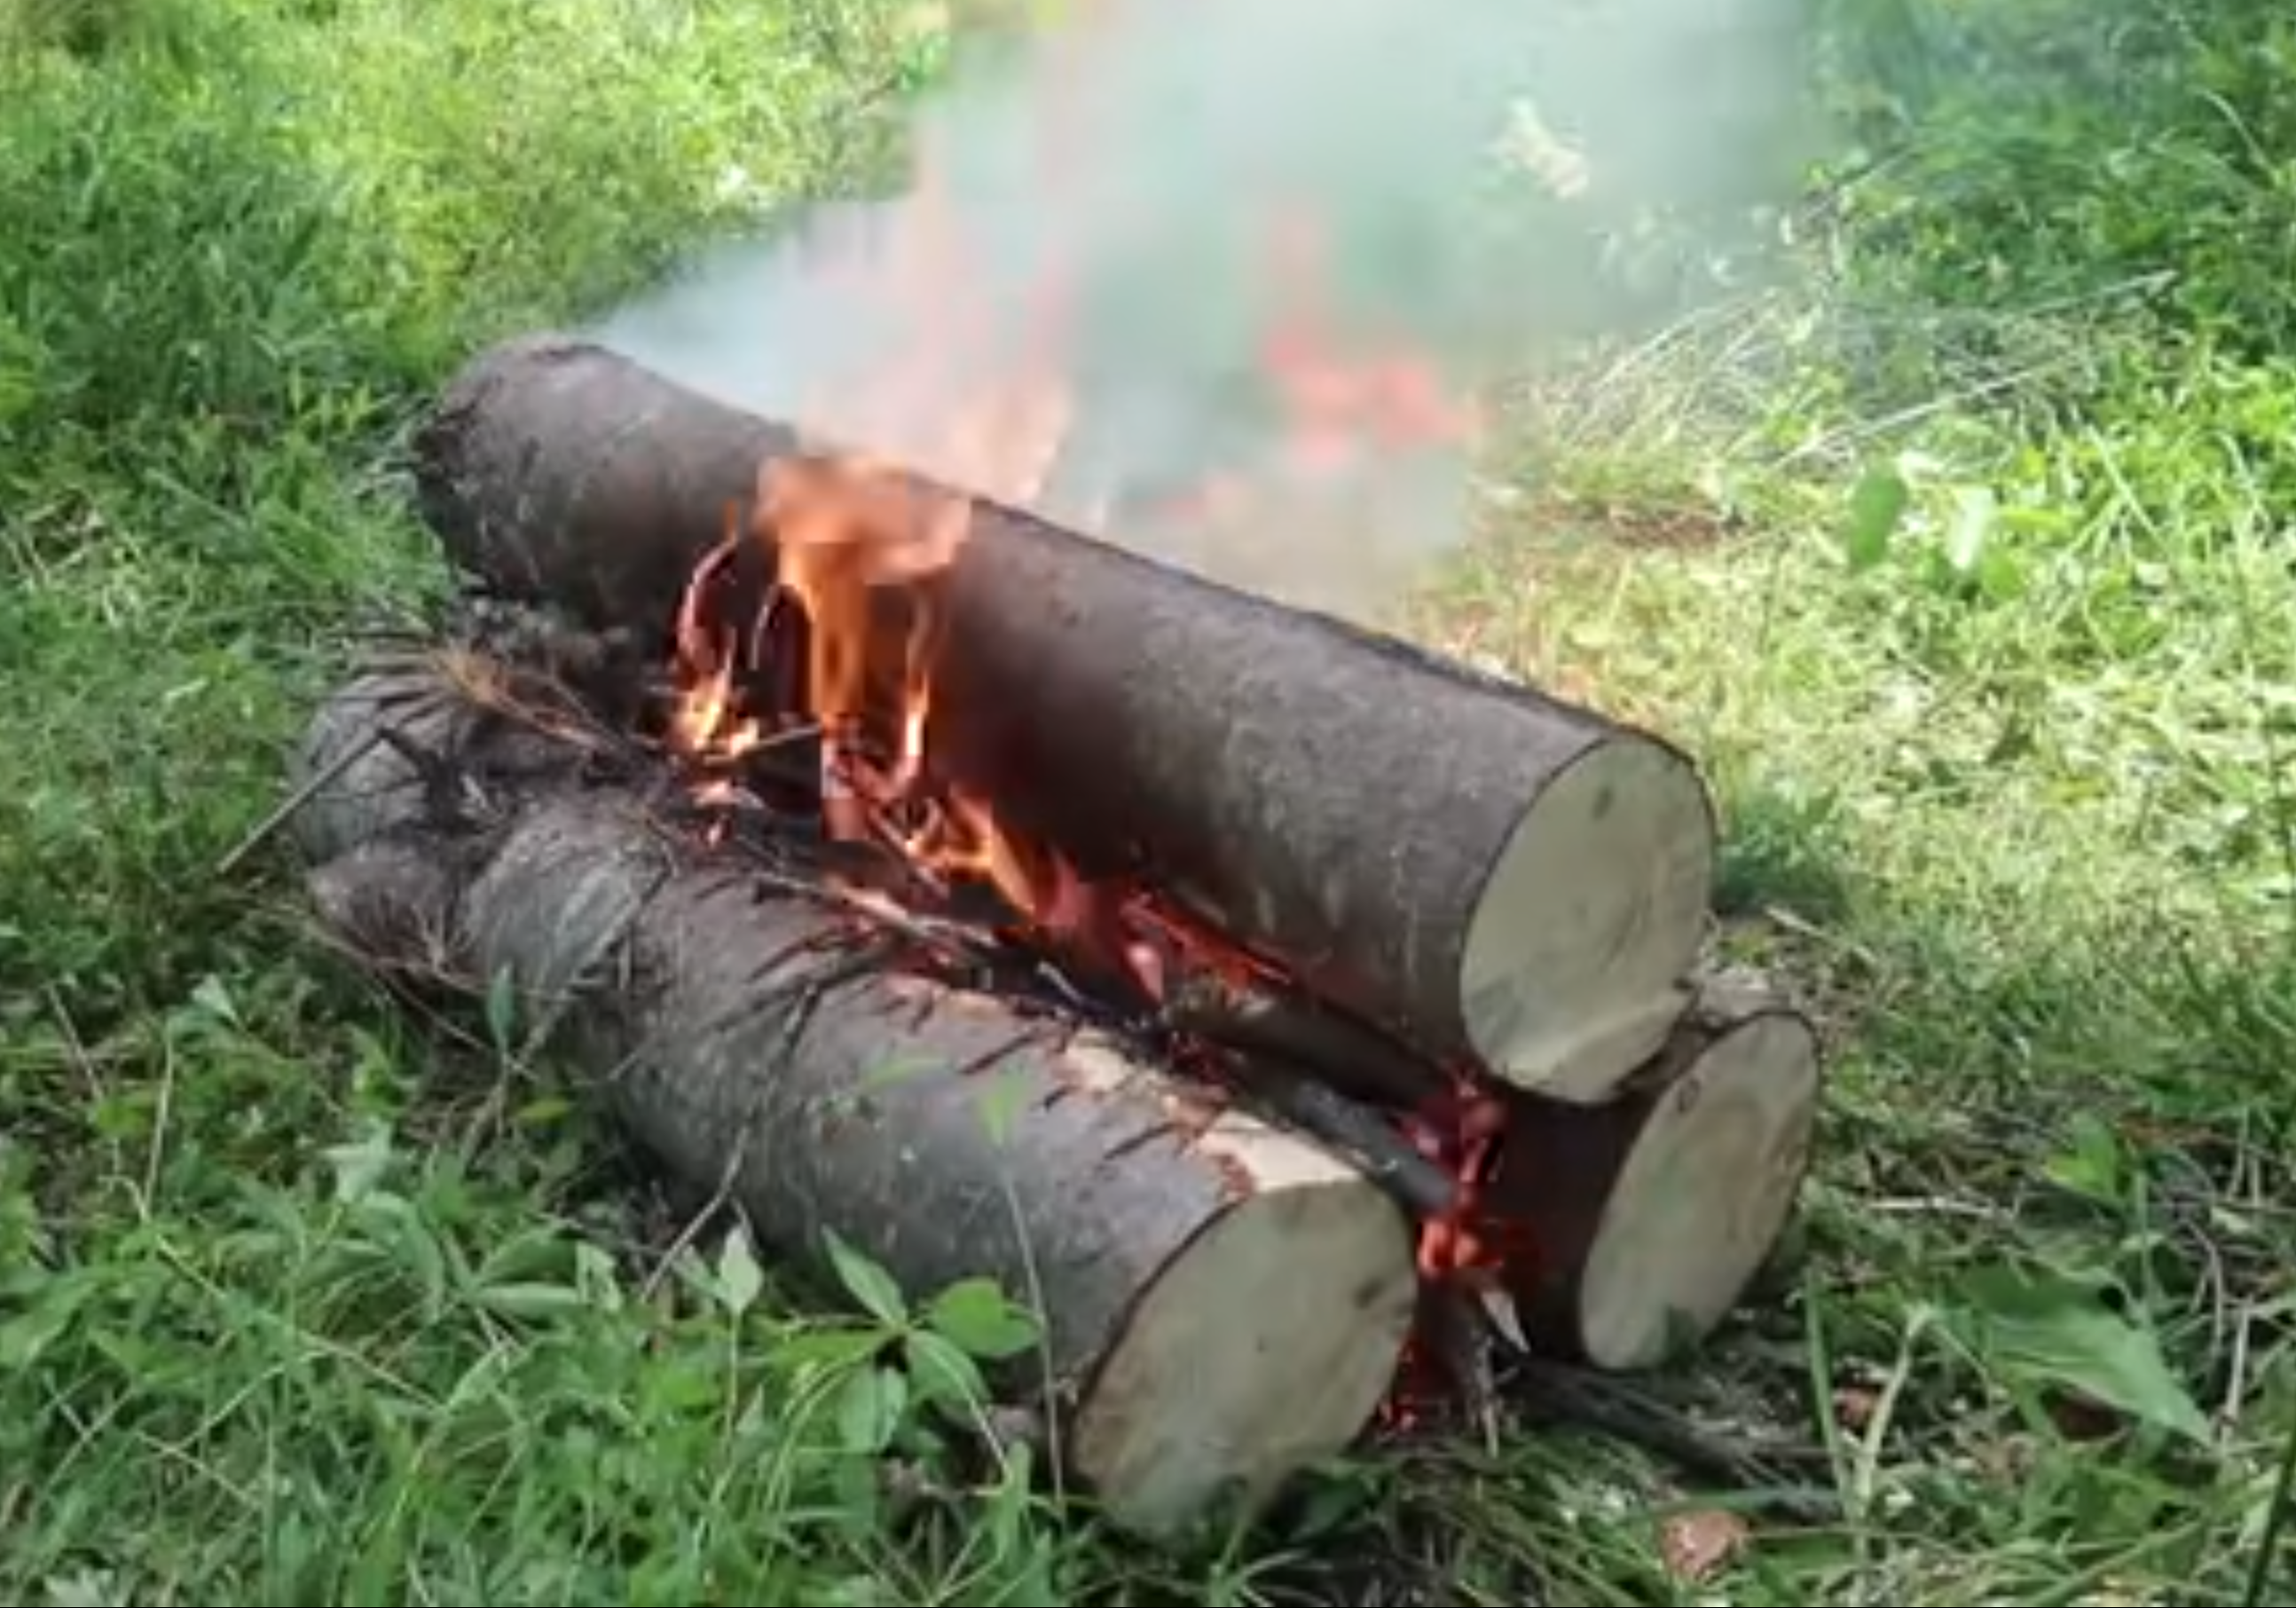
\includegraphics[height=.2\textheight]{images/three-logs.png}
    \end{center}
  }
\end{frame}
\end{document}
